\documentclass[a4paper,12pt]{extarticle}
\usepackage[utf8]{inputenc}
\usepackage[francais]{babel}
\usepackage[T1]{fontenc}
\usepackage[pdftex]{graphicx}
\usepackage{url}
\usepackage{caption}
\usepackage{multirow}

\usepackage{fancyhdr}
\pagestyle{fancy}






\setlength{\parindent}{0cm}
\setlength{\parskip}{1ex plus 0.5ex minus 0.2ex}
\newcommand{\hsp}{\hspace{20pt}}
\newcommand{\HRule}{\rule{\linewidth}{0.5mm}}
%opening

\renewcommand{\headrulewidth}{1pt}
\fancyhead[L]{\leftmark}
\fancyhead[R]{LaTeX}

\renewcommand{\footrulewidth}{1pt}
\fancyfoot[C]{\textbf{page \thepage}} 




\begin{document}

\begin{titlepage}
  \begin{sffamily}
  \begin{center}

    % Upper part of the page. The '~' is needed because \\
    % only works if a paragraph has started.
    
\includegraphics[scale=1]{univangers.jpg}~\\[1.5cm]

    \textsc{\LARGE Université d'Angers}\\[2cm]

   

    % Title
    \HRule \\[0.4cm]
    { \huge \bfseries Virtualisation d'un équipement d'une classe mobile}{\bfseries  \\[0.4cm] }

    \HRule \\[2cm]
    

    % Author and supervisor
    \begin{minipage}{0.4\textwidth}
      \begin{flushleft} \large
        CHERRUAU \textsc{Anthony}\\
        FRESNEAU \textsc{Quentin}
        POUPELIN \textsc{Bastien}\\
        THEBAUDIN \textsc{Corentin}
      \end{flushleft}
    \end{minipage}
    

    \vfill
    \HRule\\[2cm]
    % Bottom of the page
    {\large 30 Mars 2017}

  \end{center}
  \end{sffamily}
\end{titlepage}
\clearpage

\tableofcontents

\clearpage

\section{Introduction}

Au cours de notre seconde période de projet tutorés, nous avons travaillé avec M.Girardeau sur la “virtualisation d’un équipement d’une classe mobile”. Durant ce projet, nous avons dû tenir à jour une documentation didactique concernant les différentes étapes d’installation, de configuration mais aussi de résolution de problèmes auquel nous avons eut à faire.\newline
Le wiki de l’installation complète du système vient donc compléter ce rapport puisqu’il contient toutes les étapes beaucoup plus détaillés.\\

\url{http://wiki.info.univ-angers.fr/projets_etudiants:2017_l3pro_eg_virtualisation_classe_mobile}

\clearpage

\section{Présentation de l'existant}

\subsection{Contexte}
\paragraph{}
Les étudiants de la faculté des sciences de l’université d’Angers disposent d’un chariot de 40 tablettes (Samsung Galaxy Tab 4) qui permet aux étudiants, lors de travaux pratiques d’Android, d’observer leurs applications sur un support concret autre qu’un émulateur.
Lors des préparations ou aux termes des contrôles continus de cette unité, l’enseignant peut avoir besoin de déposer des fichiers, les récupérer, contrôler les répertoires, accéder aux logs et installer des applications sur les tablettes.\\

A cet effet, un projet d’étudiant de L3 informatique a été mené en 2015 afin de répondre au cahier des charges précédemment cité. Jérôme FOURMOND et Florentin NOEL ont donc développé une application pour le chariot, une application pc et une application android.\\

L’application chariot permet d’exécuter des scripts qui s’appuient sur sur le kit de développement (SDK) d’android, ADB, et qui possède les même fonctionnalités sauf qu’une marque concrète des événements produits sur la machine est enregistrée.  Elle s'exécute directement dans un terminal et  se comporte comme un serveur, elle reçoit des messages simples et exécute des les scripts associés à ces messages. L’application sert de liaison entre les tablettes et l’application PC.\\

L’application PC est une application graphique qui permet une gestion simple des tablettes connectées grâce à son interface. Les scripts sont facile à exécuter et le résultat des commandes exécutées sont affichés. \\

L’application android permet à l’utilisateur de la tablette d’obtenir des informations sur son appareil via une interface graphique claire et de commander un nettoyage de l'appareil lors de sa prochaine connexion au chariot.\\

Actuellement le chariot de tablette est composé de la sorte. Nous avons un pc principal sous pfSense qui est relié vers le wifi et l’ethernet. Ensuite nous avons un pc vertical sous xubuntu qui permet de voir les tablettes et d’utiliser les script pour des fonctionnalités sur les tablettes. Les tablettes sont reliés à deux hub usb un pour le chariot du bas et un autre pour le chariot du haut. Ces hub sont ensuite reliés au Xubuntu.\\

Le schéma ci dessous représente le chariot actuelle :\\

\begin{center}
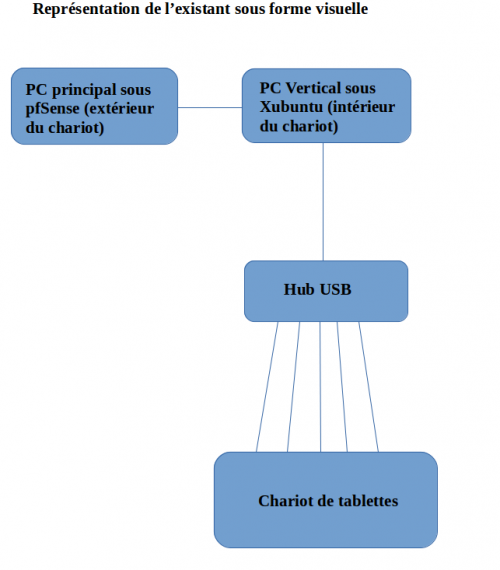
\includegraphics[scale=0.90]{representation_existant}
\end{center}

\clearpage
\subsection{Objectif du projet}

La finalité de ce projet est de permettre de n’avoir qu’un ordinateur contenant un hyperviseur de machines virtuelles, XenServer et deux machines virtuelle : le pfSense et le Xubuntu.
Cela permet de réduire le nombre de matériel requis pour le chariot. Ainsi, au lieu d’utiliser deux ordinateurs, tout est pilotable depuis un seul ordinateur et donc plus facile à gérer. De plus, on peut prévoir de futures évolutions avec l’ajout d’autres machines virtuelles en fonction des besoins des utilisateurs.

Le schéma ci dessous représente le chariot désiré :\\

\begin{center}
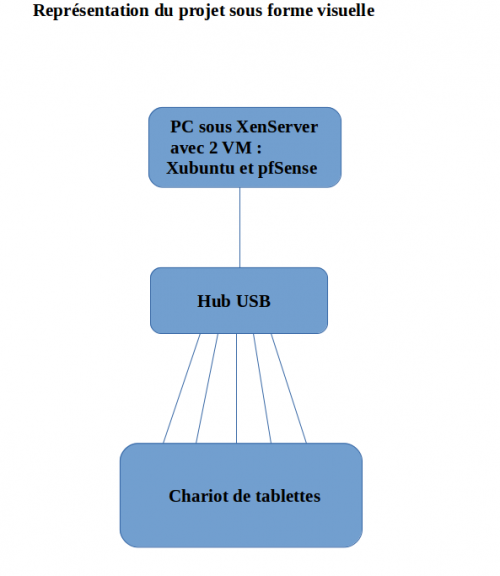
\includegraphics[scale=0.90]{representation_projet}
\end{center}

\clearpage
\section{Elaboration du projet}
\subsection{Partage du projet}

\paragraph{}
Concernant ce projet, nous avons séparé celui-ci de deux façons : la première étant l’installation et la seconde étant la recherche. En effet lors des phases d’installation, 
chacun cherchait de son côté les différentes manières d’installer les différentes machines virtuelles mais aussi de leur configuration. Suite à ces installations, nous étions souvent amenés à chercher des solutions aux différents problèmes que l’on rencontrait (voir problèmes).

\subsection{Partage du travail(GANTT)}

Pour partager le travail nous avons défini des axes et avons réparti les tâches. Nous avons donc réalisé un diagramme de Gantt qui permet de voir où l’on en était et ce qu’il reste à faire (voir annexe 1).\\
La plus grande partie des travaux réalisés durant le projet ont été des travaux de recherche pour comprendre le fonctionnement ou tout simplement résoudre les problèmes rencontrés. 
Les tâches tel que les installations ont été difficile à répartir puisque nous ne disposions que d'une seule machine. Un des grands axes du projet à aussi été la réalisation de wiki.

\subsection{Matériel à disposition}

Pour mener à bien l’ensemble du projet, M. Éric Girardeau nous a mis a disposition du matériel. Au début du projet nous avions à notre disposition :
\begin{itemize}
\item Ordinateur portable HP EliteBook 8540w, i5M560, 4Go de ram
\item Un adaptateur HP USB/Ethernet
\item Une clé USB 2.0 de 4Go
\item Une tablette Samsung galaxy tab
\item Une tablette Asus\\
\end{itemize}

Au fur et à mesure de l’avancement de notre projet nous avons rencontrés quelques problèmes matériels. C’est pour cela que de nouveaux matériels ont été mis à notre disposition :
\begin{itemize}
\item Ordinateur portable HP EliteBook 8560w, i7-2620M, 8Go
\item Un adaptateur Apple USB/Ethernet
\item Un mini hub USB 3 port (brancher 2 tablettes)
\end{itemize}

\clearpage

\subsection{Réalisation du wiki}

L’une des consignes du projet était aussi de réaliser une page wikipédia contenant les étapes clés du projet, des tutoriels d’installation ou de résolution de problèmes et l’avancement de projet.\newline
Notre tuteur nous a donc ouvert une section sur le wikipédia de l’université d’angers associant nos noms pour obtenir les droit d’écriture.\\

\url{http://wiki.info.univ-angers.fr/projets_etudiants:2017_l3pro_eg_virtualisation_classe_mobile}

\clearpage

\section{Mise en place de l'installation}
\subsection{XenServer}
\paragraph{Présentation\\}


XenServer est un logiciel libre de virtualisation, ou plus précisément un hyperviseur de machine virtuelle basé sur centOS.\\

Xen permet d'exécuter plusieurs systèmes d'exploitation (et leurs applications) de manière isolée sur une même machine physique sur un grand nombre de plate-formes. Les systèmes d'exploitation invités partagent ainsi les ressources de la machine hôte.\\

Xen est un « paravirtualiseur » ou un « hyperviseur » de machines virtuelles. Les systèmes d'exploitation invités ont « conscience » du Xen sous-jacent, ils ont besoin d'être « portés » (adaptés) pour fonctionner sur Xen. Linux, NetBSD, FreeBSD, Plan 9 et GNU Hurd peuvent d'ores et déjà fonctionner sur Xen.\\

\paragraph{Dans le projet\\}

Pour débuter le projet, le choix de l’hyperviseur Xen à été fait en fonction des consignes de notre tuteur mais il aurait été possible d’utiliser d’autres logiciels libres gratuit équivalent tel que Proxmox. \\
Les premiers tests ont été réalisés avec la version 7.0 de XenServer. L’installation se fait classiquement par le biais d’un ISO sur une clé USB bootable.

\begin{center}
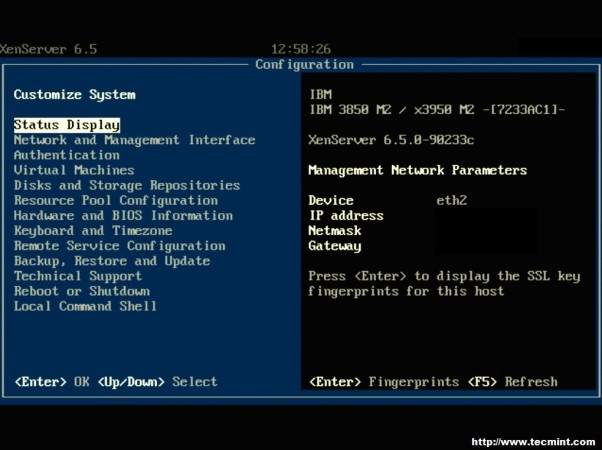
\includegraphics[scale=0.60]{xenserver18}\\
\end{center}

L’interface est plutôt sobre et ne permet que quelques fonctionnalités simples comme le changement d’adresse IP ou le redémarrage de machines virtuelles etc. Afin de pouvoir réaliser des opérations complexes comme la création d’une machine virtuelle, il faut utiliser les lignes de commandes ou un client externe dont nous parlerons dans la partie d de ce projet.\\

Les lignes de commande sont toutefois essentielles pour certaines fonctionnalités comme l’attribution d’un port USB à une machine virtuelle définit. Dans notre cas, la machine virtuelle Xubuntu devait pouvoir accéder à au moins 1 port USB pour être relié aux hub du chariot.

\subsection{PfSense}
\paragraph{Présentation\\}

PfSense est un routeur/pare-feu open source. Il utilise le pare-feu à états Packet Filter, des fonctions de routage et de NAT lui permettant de connecter plusieurs réseaux informatiques. Il comporte l'équivalent libre des outils et services utilisés habituellement sur des routeurs professionnels propriétaires. pfSense convient pour la sécurisation d'un réseau domestique ou de petite entreprise.


\paragraph{Dans le projet\\}

Cette machine virtuelle va nous permettre de faire le lien entre le WAN et le LAN. Le PfSense a deux interfaces réseaux : une qui est la carte réseau de l’ordinateur et l’autre qui est l’adaptateur USB/Ethernet. Le PfSense va permettre à Xubuntu d’avoir un lien vers l’extérieur pour que les tablettes aient un accès au WAN. \newline
PfSense est à la version 2.3.2 qui, au moment de l’installation, était la dernière version stable. Mais une nouvelle version est apparu entre-temps la 2.3.3 mais nous n’avons pas mis à jour notre pfSense pour autant. Il y a donc une évolution de Pfsense possible.  

\begin{center}
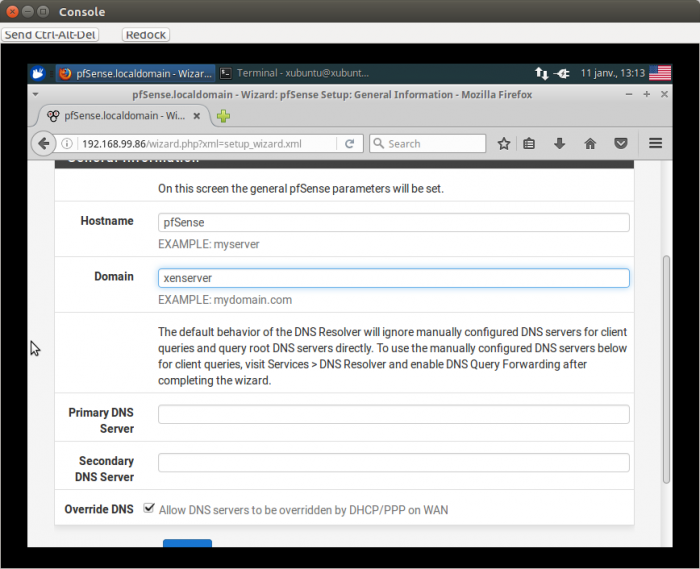
\includegraphics[scale=0.65]{pfsense}\\
Page de connexion de pfSense
\end{center}
\paragraph{}
PfSense peut être piloté par une interface web accessible depuis la machine virtuelle Xubuntu. La configuration s’est faite via le fichier de configuration de pfSense utilisé sur l’ancienne version du chariot.\\


\paragraph{}
\begin{table}[!h]
\begin{tabular}{|p{3cm}|p{3cm}|p{3cm}|p{3cm}|}
\hline
 & Configuration minimale & Configuration recommandée & Configuration choisie\\
\hline 
Processeur & 500 MHz & 1 GHz & 512 MHz\\
\hline
Mémoire vive & 512 Mo & 1 Go & 512 Mo \\
\hline
Stockage & >1 Go & & 15 Go \\
\hline
\end{tabular}
\caption{Configuration de pfsense}
\end{table}


\subsection{Xubuntu}
\paragraph{Présentation\\}

Xubuntu est un système d'exploitation libre de type GNU/Linux. C'est un projet issu de la Fondation Ubuntu utilisant l'environnement de bureau graphique Xfce à la place d'Unity. Le projet Xubuntu est une distribution Linux dérivée de Ubuntu, car tous deux partagent exactement la même base, des logiciels communs (Synaptic), les mêmes dépôts APT, le même nom de code et le même cycle de développement.


\paragraph{Dans le projet\\}

Dans le cadre de notre projet, nous utilisons la versions Xubuntu 16.04 Xenial Xerus qui est la dernière version de Xubuntu. C’est une version 64 bits puisque les scripts développés par les étudiants (en 2015) sont adaptés pour une machine en 64 bits.
Le choix de xubuntu est dû au fait que c’est un version plus légère de linux et cela permet sur une machine virtuelle d’économiser les ressources et d’avoir une machine virtuelle plus stable.
Le xubuntu va nous permettre de voir les tablettes et d’utiliser les script de gestion des tablettes. \\
Le choix de Xubuntu était imposé dès le début du projet car en prenant une Ubuntu( par exemple), il y aurait eu  un problème sur le nombre de tablette détecté par Ubuntu. La prise en charge de multiples matériels sur un USB est bloqué à sept sur Ubuntu d'où le choix de Xubuntu pour voir nos 42 tablettes. 
Pour le fonctionnement des scripts le kit de développement (SDK) d’android ADB a été ajouté à la machine.

\paragraph{\\}
\begin{table}[!h]
\begin{tabular}{|p{3cm}|p{3cm}|p{3cm}|p{3cm}|}

\hline
 & Configuration  minimale & Configuration recommandée & Configuration choisie\\
\hline 
Processeur & 750 MHz & 1,6 GHz & 1,6 MHz\\
\hline
Mémoire vive & 512 Mo & 2 Go & 2 Go \\
\hline
Stockage & 8 Go & 16 Go & 30 Go \\
\hline
\end{tabular}
\caption{Configuration de Xubuntu}
\end{table}

\subsection{OpenXenManager}

\paragraph{}
Travaillant sous Linux il nous fallait un logiciel pouvant se connecter à notre serveur Xen en ayant une interface graphique de nos machines virtuelles. Sous linux le seul logiciel est openXenManager qui est un logiciel officiel pour un serveur Xen. Ce dernier permet d’effectuer des actions sur l’hyperviseur et ses machines virtuelles mais aussi d’utiliser les interfaces graphique des différentes machines virtuelles sous le XenServer. 
On peut par exemple créer des machines virtuelles, les stopper, les redémarrer. Une alternative à OpenXenManager existe sous Windows nommé XenCenter, on a dû aussi l’utiliser au cours du projet afin d’installer les tools manquants.

\begin{center}
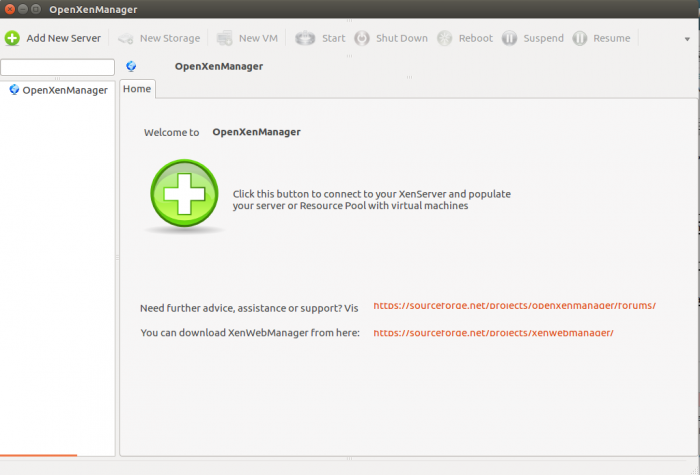
\includegraphics[scale=0.70]{openxenmanager}
\end{center}

\section{Etat final du projet}
\subsection{Présentation final du système}

\paragraph{}
Dans notre projet final, nous avons mis en place serveur Xen sur un PC portable (avec XenServer) qui contient les machines virtuelles PfSense et Xubuntu. PfSense a deux cartes réseaux, celle de l’ordinateur pour le LAN et l’adaptateur USB/Ethernet pour le WAN. Deux ports USB de l’ordinateur sont vu par le Xubuntu. En reliant l’ordinateur au chariot, les 42 tablettes n’étaient pas forcément toutes détectées par Xubuntu. 
En effet, quand on branchait les tablettes, un message s’affichait sur chacune d’entre elles. Il fallait alors l’accepter pour autoriser la communication entre l’ordinateur et les tablettes. Il fallait aussi vérifier que le mode débogage soit bien actif sur les tablettes pour avoir ce message mais aussi pour pouvoir lancer les différents scripts par la suite. Nous pouvons utiliser le script des gestions de tablettes pour vérifier le nombre de tablettes connectées et celles qui n’y sont pas. \\

Le projet final est représenté par le schéma ci dessous :

\clearpage
\paragraph{Schéma du chariot détaillé}
\begin{center}
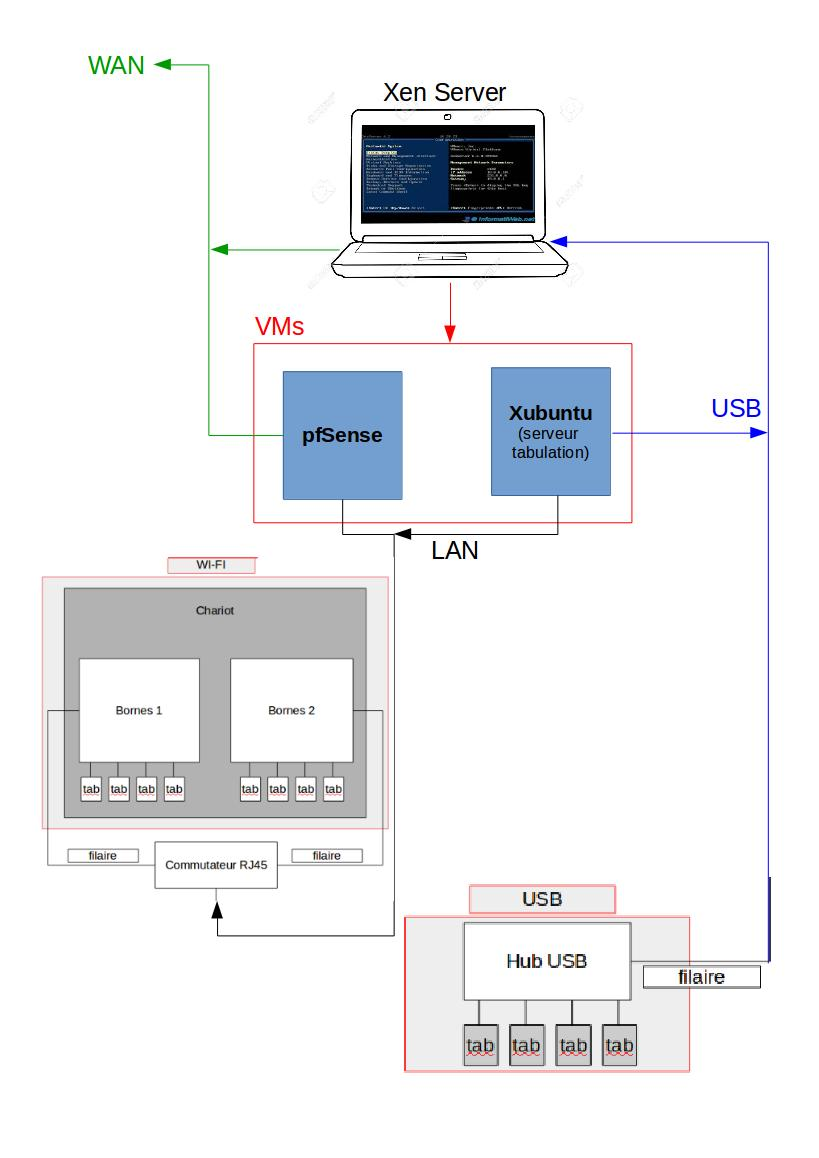
\includegraphics[scale=0.65]{chariot}\\
\end{center}

\subsection{Améliorations}

\paragraph{}
Il y a plusieurs axes d’améliorations possibles. \\
Tout d’abord celui de gérer les bornes wifi depuis PfSense. Il y a déjà une configuration de faite mais pour mettre à jour une configuration de pfSense celui-ci doit avoir accès à internet. Pour cela, M.Girardeau donnera un accès direct au réseau de la fac (sans authentification) pour le PfSense. Cela permettra donc de mettre à jour la configuration de pfSense et que les bornes wifi soit prises en compte.\\ 

Ensuite pour avoir accès à toutes les machines sur un ordinateur il faudrait mettre XenServer en machine virtuelle (sous Virtualbox par exemple) et ensuite créer les machines virtuelles PfSense et Xubuntu depuis le XenServer. On pourrait ensuite accéder directement depuis le même ordinateur a toutes les machine virtuelles. Néanmoins, ce genre d’installation demanderait un ordinateur un peu plus puissant (surtout en terme de mémoire).


\clearpage
\section{Problèmes rencontrés}

\subsection{Problèmes matériels}

Au cours du déroulement du projet, nous avons dû faire face à différents problèmes aussi bien d’installation, de configuration, de logiciel ou bien même de matériel. Face à ces problèmes, nous avons décidé de d’abord lever des hypothèses, puis réaliser des tests pour enfin en trouver la/les solution(s).\\

L’un des problèmes les plus imposants était lors du test de la reconnaissance de la tablette, elle n’était pas reconnue par la machine virtuelle Xubuntu. En effet, une fois que nous avions réussi à installer et faire fonctionner le système, nous avons tenté de brancher une tablette sur un port USB.\newline
Nous avons donc d’abord levé des hypothèses. La première d’entre elles était que le protocole MTP (connexion des appareils Android par USB) n’était pas géré par le noyau de Linux ou de Xen. La seconde était que le port USB n’était peut-être pas monté.
À force de recherches et de différents tests, nous avons trouvé que pour pouvoir utiliser les ports USB et que les tablettes soient reconnus sur la machine virtuelle Xubuntu, il fallait que le port USB soit associé à la machine virtuelle.\\


Pour cela, nous avons utilisé différentes commandes dont voici la liste :\\

\paragraph{Reconnaissance de la tablette de test\\}

La tablette n’était pas reconnu par la machine virtuelle Xubuntu.

Hypothèse :
\begin{itemize}
\item Protocole MTP (connexion des appareils android par USB) non géré par le noyau de linux de XEN
\item Le port USB n’est peut être pas monté \\
\end{itemize}

Solution :
Pour pouvoir utiliser les ports usb et que les tablettes soient reconnus sur la vm Xubuntu il faut que le port usb soit associé à la vm. 

lister les port USB et leur ID pour recuperer l'ID du port USB qui nous intéresse :
\begin{verbatim}
lspci
\end{verbatim}
Ainsi, on peut identifier le port que l’on veut associer à la machine virtuelle et récupérer son ID.\\
On liste les machines virtuelles et leur UUID pour récupérer l’UUID qui nous intéresse :
\begin{verbatim}
xe vm-list
\end{verbatim}

Associer UUID et ID :
\begin{verbatim}
xe vm-param-set other-config:pci=”ID” uuid=”UUID”
\end{verbatim}
Ainsi, les ports USB étaient débloqués et utilisables.



\paragraph{Reconnaissance de l'ensemble des tablettes\\}
Seulement 13 tablettes sur 40 de reconnu lors d'essai sur le chariot

Hypothèse :
\begin{itemize}
\item Test réalisé hors tension, peut être pas assez de courant pour pouvoir alimenté tous les ports USB ? 
\item Toutes les tablettes sont-elles en mode débogage ? 
\item Le noyau ou la configuration du noyau de l'ordinateur permet t'il de voir un nombre limité de tablettes ? \\
\end{itemize}

Test :
\begin{itemize}
\item Branchement de l'ordinateur sur secteur. NON CONCLUANT
\item Test de débranchement d'une tablette, une autre est prise en compte. NON CONCLUANT \\
\end{itemize}

Solution :
Problème de matériel : Alimentation fournit par le port USB pas assez importante. 
Nouvel ordinateur fournit.


\subsection{Problèmes logiciels}


\paragraph{Decouverte des ISOs lors de l'installation de VM\\}
Lors de l'installation des VMs via openXenManager, après transfert des ISOS, ceux-ci demeurent introuvable dans l'explorateur de fichiers.

Hypothèse :
\begin{itemize}
\item problème d'update de l'affichage des fichiers de OpenXenManager\\
\end{itemize}

Solution :
Transfert via SSH des ISOs puis reboot de XenServer.\\


\clearpage

\section{Conclusion}
Ce projet nous a été proposé par M. Éric Girardeau lors de la seconde période de projets tutorés. Dans ce projet, nous devions mettre en place un serveur Xen sur un PC (de préférence portable) avec deux machines virtuelles. L’une d’elles sert de passerelle PfSense et devra pouvoir importer une configuration existante et l’autre sous Xubuntu qui intégrera le serveur de gestion des tablettes du chariot.\\

Aujourd’hui, nous pensons répondre aux attentes finales du projet c’est-à-dire de pouvoir gérer le chariot de tablettes avec un serveur Xen sur un seul ordinateur. En effet, nous avons réussi à avoir accès à l’ensemble des tablettes ainsi que de lancer les différents scripts permettant la gestion des tablettes.\newline
Il reste néanmoins quelques modifications possibles pour compléter notre réalisation.
Tout d’abord, il serait possible de donner accès à Internet au PfSense afin de pouvoir y importer des configurations existantes. Ensuite, il serait possible de tout regrouper sur un seul ordinateur d’une différente manière. Pour cela, il suffirait d’installer directement XenServer sous forme de machine virtuelle (avec par exemple VirtualBox) : une machine virtuelle sous XenServer, et ce XenServer contenant les deux VM sous PfSense et Xubuntu.\\

Ce projet contenait deux principales phases. Une phase d’installation/ configuration et une de recherche de solutions lorsque nous étions confrontés à des problèmes.
À l’issue de ce projet, nous avons pu travailler en équipe pour essayer de compléter les recherches de chacun. Même si l'intérêt premier des projets tutorés est de mettre à profit ses connaissances afin d’en développer de nouvelles, le fait de travailler directement sur le chariot de tablettes nous a poussés à fournir au final un système qui répond aux conditions et aux attentes de M.Girardeau. Ce projet a donc été intéressant pour tout le groupe puisque notre production a pu être testée et observée sur un cas concret, ce qui nous a donc motivé à rendre ce projet fonctionnel à temps. 

\clearpage
\section{Références}

Informations/Installation PfSense, Xubuntu et XenServer :

\url{https://fr.wikipedia.org/wiki/Xen}\\
\url{https://fr.wikipedia.org/wiki/Pfsense}\\
\url{http://www.sky-future.net/wp-content/uploads/2015/01/Installation+pfSense.pdf}\\
\url{https://services.renater.fr/ntp/serveurs_francais}\\

Installation/Lancement script Android :

\url{http://www.informatiweb-pro.net/virtualisation/1-citrix/15--citrix-xenserver-pci-passthrough--2.html}\\
\url{https://doc.ubuntu-fr.org/androiddebugbridge}\\
\url{https://launchpad.net/~nilarimogard/+archive/ubuntu/webupd8}\\

Réseau PfSense/XenServer/Xubuntu :

\url{https://support.citrix.com/article/CTX121615}\\

USB XenServer :

\url{https://medium.com/@alexander.bazhenov/\%D0\%BF\%D1\%80\%D0\%BE\%D0\%B1\%D1\%80\%D0\%BE\%D1\%81-usb-\%D1\%83\%D1\%81\%D1\%82\%D1\%80\%D0\%BE\%D0\%B9\%D1\%81\%D1\%82\%D0\%B2-\%D0\%B2-xenserver-50a9b4e8a80a#.icnppyde6}\\
\url{http://www.informatiweb-pro.net/virtualisation/1-citrix/15--citrix-xenserver-pci-passthrough--2.html}\\

Adaptateur ethernet :

\url{https://lists.xenproject.org/archives/html/xen-api/2013-07/msg00038.html}\\
\url{https://support.citrix.com/article/CTX121615}\\

\clearpage

\section{Annexes}

GIT du projet :
\url{https://github.com/acherruau/projet2}\\

Wiki de la réalisation du projet :\\ 
\url{http://wiki.info.univ-angers.fr/projets_etudiants:2017_l3pro_eg_virtualisation_classe_mobile}\\

\begin{center}
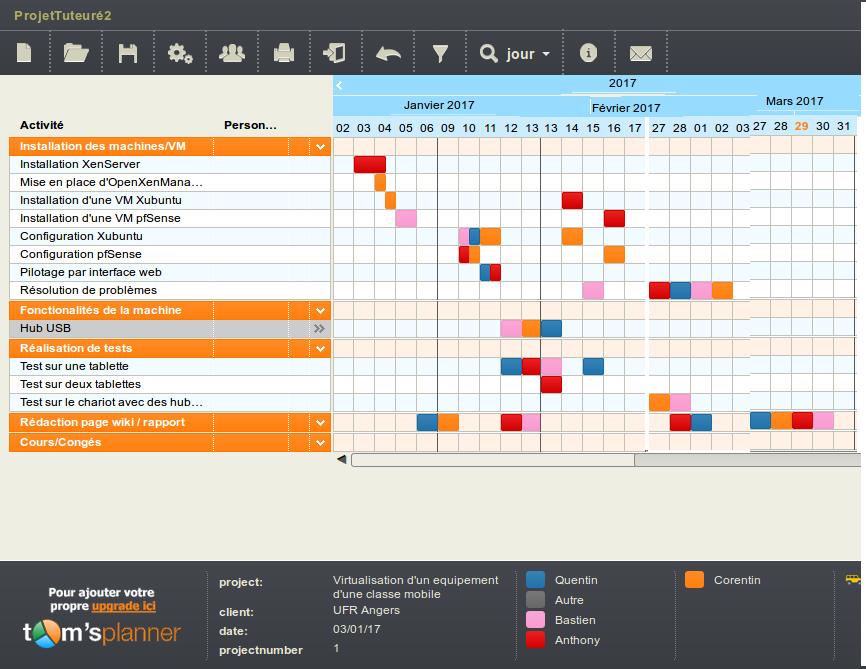
\includegraphics[scale=0.6, angle=270]{Gantt4}
\end{center}

\end{document}
\newline


